\section{related work} \label{sec.relatedwork}
Scientists proposed many methods based on lung volume, gas sensing, and imaging~\cite{Lorenzo:2013}.
In terms of lung volume methods, peak expiratory flow (PEF) is the most commonly used parameter for monitoring lung function of asthma patients. It is very popular in primary care because it can be measured easily by simple, cheap and portable devices. Forced Expiratory Volume in 1 Second (FEV$_1$) is also a widely used standard for  measuring airflow caliber. However, methods measuring these two parameters have some common limitations: lack of compliance, possible falsification of results, and long recording periods~\cite{Moscato:1995}.
Gas sensing method is another sensing modality to detect asthma by monitoring Nitric oxide (NO) and CO$_2$. NO gas level will increase when asthma attack occurs~\cite{Kharitonov:1994}. The CO$_2$ output patterns between healthy and asthma-suffering patients are different~\cite{You:1994}.
Furthermore, with the development of sophisticated imaging techniques, image of lung in asthma patients has evolved dramatically over decades, such as positron emission tomography (PET), magnetic resonance imaging (MRI), single photon emission computed tomography (SPECT), and ultrasound (US). These techniques provide different approaches to visualize gross anatomic abnormalities, regional lung mechanics, and airway anatomy. They are also very useful for understanding the different functions between the lungs of healthy subjects versus asthma patients~\cite{Mario:2011}.
Compared with these oneshot images methods, ultrasound method can capture image sequences of moving organs and tissues, which enables users perform real-time analysis of respiration via ultrasound imaging technology. Better portability and no radiation are another two advantages of ultrasound sensing modality. Thus, it will be safer for long-time monitoring and can be used with special group of people, such as pregnant women and children.
\begin{figure*}[htb]
\centering
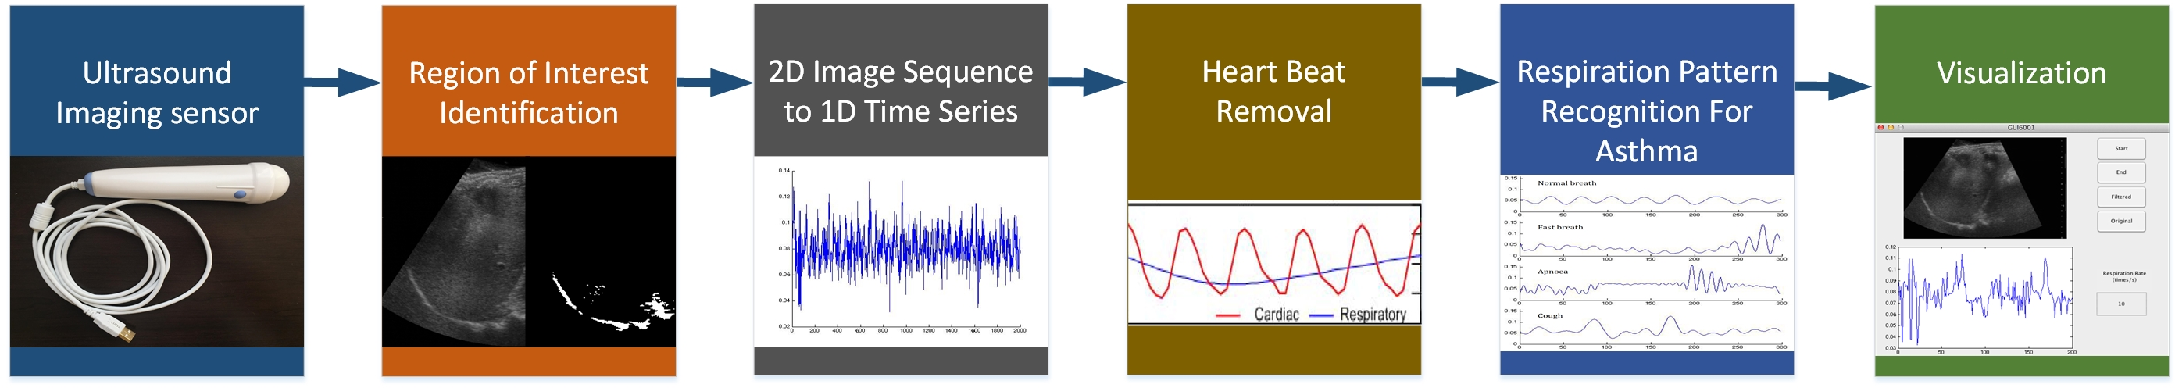
\includegraphics[width=1\textwidth]{Framework.pdf}
\caption{Overview of the ultrasonography processing procedures}
\label{fig.System}
\end{figure*}

There are many proposed approaches to detect respiratory motions based on ultrasound devices. Bruin et al.~\cite{Bruin:1997} found that asthma patients had thinker $D_iT_{relax}$, diaphragm thickness during relaxation. So they measured $D_iT_{relax}$ from B-mode ultrasound images to detect asthma patterns.
Researchers also could infer respiration pattern by quantifying the movements of a kidney, because kidney moves along with breathing~\cite{Laurent:1994}. According to research of Wachinger et al.~\cite{Christian:2011}, the neighborhood relationship of organs is related with breathing cycle. They measured respiration by investigating 2D ultrasound images of liver and kidney. This method has the advantage that it is fully automatic and does not require a training phase or prior information about underlying anatomy, nor the interaction of user.
Tuathan et al.~\cite{Tuathan:2014} proposed a 2D normalized cross-correlation (NCC) based algorithm to estimate movement of a liver in 2D ultrasound images. But, due to the blur boundaries of kidney and liver in low contrast ultrasound image, the performance of  monitoring still requires further improvement.
In 2006, Xu et al.~\cite{Xu:2006} proposed a novel respiratory detection method based on diaphragm motion using a 2D ultrasound unit. Because white diaphragm region in ultrasound image is outstanding among  dark regions of organs, their method could easily extract respiratory signal from an automated analysis of the internal diaphragm movement during breathing. They selected the region of interest (ROI) and computed the mutual information (MI) and correlation coefficient (CCs) between reference ultrasound frame and all other frames. From their experiments, they discovered that MI and CC values produced a 1D signal corresponding to the respiratory cycle in both phase and magnitude.
In 2012, Hwang et al.~\cite{Youngkyoo:2012} proposed a system that placed feature windows on ROI of each ultrasound image and calculated organ's displacement through feature windows. Their proposed method can robustly extract respiratory motion signal with regardless of reference frame, because this method computed actual organ's displacement instead of similarity measurement like MI or CC. This method could provide clear information of the phase of respiratory cycle such as inspiration and expiration. The drawback of Hwang's approach is that adaptive thresholding algorithm implemented in his paper cannot detect diaphragm region robustly.

In this paper, we propose a system to perform analysis of respiration, which implements Chan-Vese algorithm to segment the diaphragm area from ultrasound image sequence accurately and identifies respiratory signals corresponding to diaphragm activities. To reduce the interference of cardiac motion, this system performs low-pass filter to purify time-series signals. Furthermore, in order to detect asthma attack by monitoring irregular breathing symptoms, we identify one normal breathing template and three irregular templates related to the three symptoms of asthma attack: frequent cough, breathing faster than normal, and shortness of breath. By comparing with these four templates, the proposed system can detect irregular respiratory patterns and notify asthma attack occurrence. 